\documentclass[xcolor=x11names,compress]{beamer}
\usepackage[english]{babel}

%% General document %%%%%%%%%%%%%%%%%%%%%%%%%%%%%%%%%%
\usepackage{graphicx}
\usepackage{tikz}
\usepackage{wrapfig}
\usepackage{hyperref}

\usetikzlibrary{decorations.fractals}
%%%%%%%%%%%%%%%%%%%%%%%%%%%%%%%%%%%%%%%%%%%%%%%%%%%%%%


%% Beamer Layout %%%%%%%%%%%%%%%%%%%%%%%%%%%%%%%%%%
\useoutertheme[subsection=false,shadow]{miniframes}
\useinnertheme{default}
\usefonttheme{serif}
\usepackage{palatino}

\setbeamerfont{title like}{shape=\scshape}
\setbeamerfont{frametitle}{shape=\scshape}

\setbeamercolor*{lower separation line head}{bg=DeepSkyBlue4} 
\setbeamercolor*{normal text}{fg=black,bg=white} 
\setbeamercolor*{alerted text}{fg=red} 
\setbeamercolor*{example text}{fg=black} 
\setbeamercolor*{structure}{fg=black} 
 
\setbeamercolor*{palette tertiary}{fg=black,bg=black!10} 
\setbeamercolor*{palette quaternary}{fg=black,bg=black!10} 

\renewcommand{\(}{\begin{columns}}
\renewcommand{\)}{\end{columns}}
\newcommand{\<}[1]{\begin{column}{#1}}
\renewcommand{\>}{\end{column}}
%%%%%%%%%%%%%%%%%%%%%%%%%%%%%%%%%%%%%%%%%%%%%%%%%%
\newcommand{\hlb}[1]{\textbf{\textcolor{blue}{#1}}}
\newcommand{\hl}[1]{\textcolor{blue}{#1}}
\newcommand{\lien}[2]{\mathcal{L}_{#1}^{#2}}
\newcommand{\lie}[1]{\mathcal{L}_{#1}}

\newcommand{\colv}[2]{\begin{pmatrix}#1\\#2\end{pmatrix}}

%\usepackage[english]{babel}
\usepackage[utf8]{inputenc}
%\usetheme{Goettingen}

\begin{document}
\title{Bifurcations in continuous time dynamical systems}
\author{Debsankha Manik}

\begin{frame}

%opening

\titlepage

\end{frame}
\section{Transient chaos}

\begin{frame}{Hard impact in an oscillating system}
\begin{figure}
\caption{}
\begin{center}
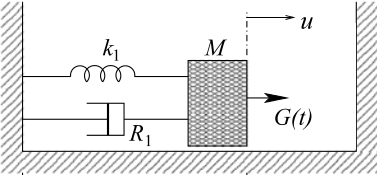
\includegraphics[width=0.4\columnwidth]{hardcol}
\end{center}
\end{figure}

The equation of motion:
\begin{equation}
\label{eq:driven}
\ddot{x}+\gamma\dot{x}+\omega_0^2x=F\cos{\omega t}
\end{equation}

Switching manifold:
If $x=\sigma$,
\begin{eqnarray*}
x&\mapsto& x\\
v&\mapsto& -v
\end{eqnarray*}
\end{frame}

\begin{frame}
The solution to equation \eqref{eq:driven} is a sum of two parts: a 
\emph{particular solution} that is independent of the initial conditions, and 
a \emph{homogeneous solution} that is dependent on the initial conditions.  

To be more precise:
\begin{eqnarray*}
x_p(t)&=&\frac{F}{\sqrt{(\omega_0^2-\omega^2)^2+\omega^2\gamma^2}}cos(\omega t+tan^{-1}\frac{\omega \gamma}{\omega^2-\omega_0^2})\\
x_h(t)&=&\frac{e^{-\gamma t/2}}{\omega_g}\left\{(\omega_g\cos{\omega_gt}+\frac{\gamma}{2}\sin{\omega_gt})x_0 + (\sin{\omega_gt})v_0 \right\}\\
\omega_g&=&\sqrt{\omega_0^2-\frac{\gamma^2}{4}}
\end{eqnarray*}
\end{frame}

\begin{frame}
Now, $x_h(t)$ decays exponentially with time.  So, if the hard wall were not 
there, any arbitrary initial condition would have been attracted to the 
period-1 orbit 
$x_p(t)$.\\
\vspace{1em}
Therefore $x_p(t)$ is a limit cycle whose basin of attraction is the 
whole phase space (ignoring the wall).  \\

\vspace{1em}

However, we note here that the friction term $\gamma$ dictates how quickly any 
arbitrary initial condition converges to this limit cycle. \\

\vspace{1em}

The limit cycle is basically a sinusoidal orbit with amplitude $\frac{F}{\sqrt{(\omega_0^2-\omega^2)^2+\omega^2\gamma^2}}:=F_g(\omega_0,\omega,\gamma,F)$ 
\end{frame}

\begin{frame}{Bifurcation w.r.t. F}
\begin{figure}
\begin{center}
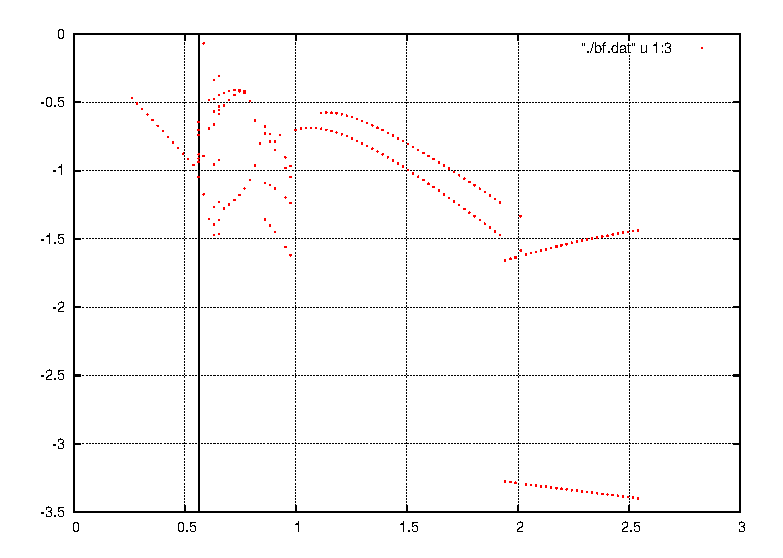
\includegraphics[width=0.9\columnwidth]{short}
\end{center}
\end{figure}
\end{frame}

\begin{frame}{A closer look}
\begin{figure}
\begin{center}
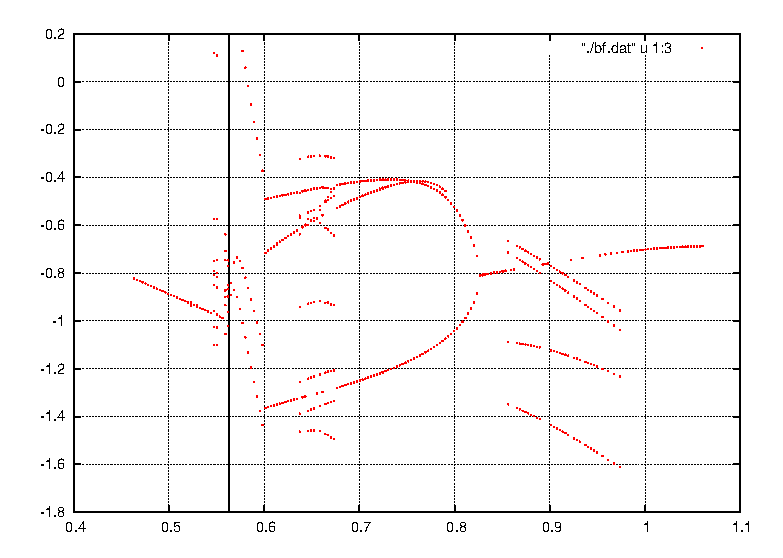
\includegraphics[width=0.9\columnwidth]{short-zoomed}
\end{center}
\end{figure}
\end{frame}

\begin{frame}{Transient behaviour}
\begin{figure}
\begin{center}
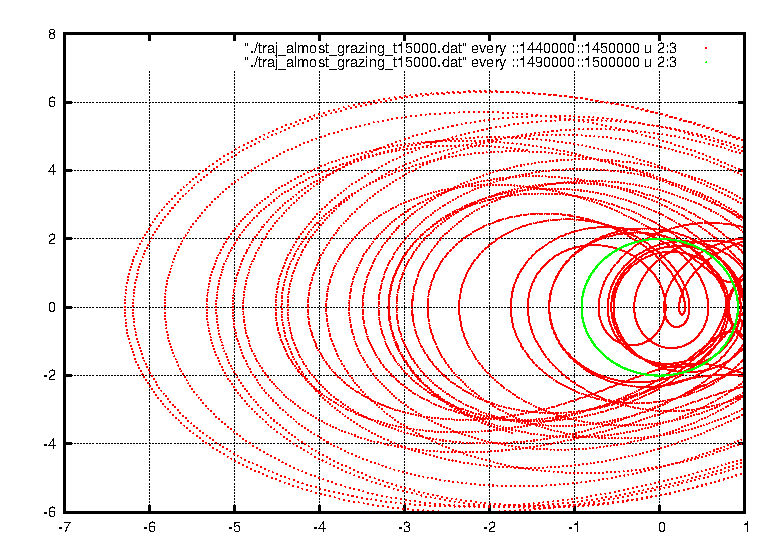
\includegraphics[width=0.9\columnwidth]{comparison-transient-chaos}
\end{center}
\end{figure}
\end{frame}

\begin{frame}
Here it needs to be emphasized that this long-lived transient is an artifact 
of the nonlinearity of the system. \\

\vspace{1em}
In this particular example, $\gamma=0.062$.  Therefore, 
$e^{-0.062\times1000/2}\approx 3.44e-14$.  \\

\vspace{1em}
The system should have settled down to the period-1 limit cycle long ago.  \\
\end{frame}

\section{Vanishing chaos}
\begin{frame}{Vanishing chaos}
When $\frac{2\omega_g}{\omega}$ is an integer, no chaos is observed at grazing:
\begin{figure}
\begin{center}
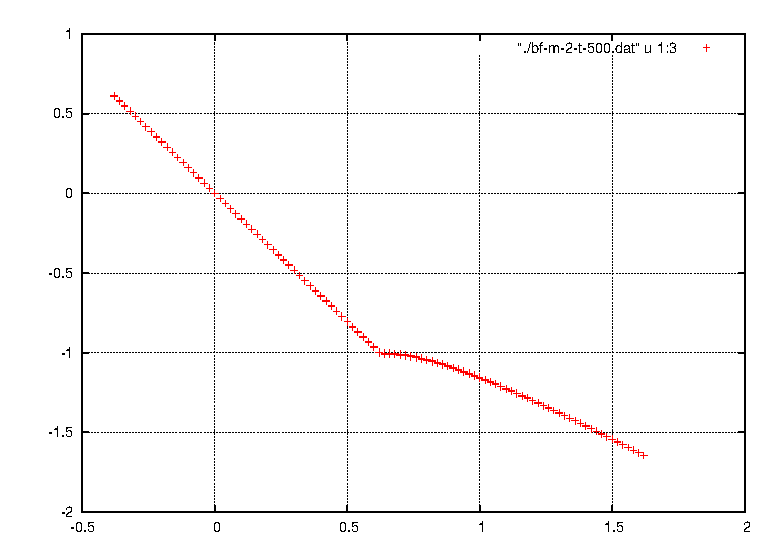
\includegraphics[width=0.9\columnwidth]{chaos-vanish-m-2}
\end{center}
\end{figure}
\end{frame}

\begin{frame}
\section{Alternate approach to ZDM}
Suppose the parameters of the system are set such that 
$\frac{F}{\sqrt{(\omega_0^2-\omega^2)^2+\omega^2\gamma^2}}=F_g(\omega_0,\omega,\gamma,F)=\sigma$
. This constitutes a steady state grazing orbit.  \\
 \vspace{1em}

Suppose we look at stroboscopic time slices such that the grazing orbit grazes 
the boundary at $t=\tau$.  \\
\vspace{1em}

Now we perturb the system slightly so that the system hits the boundary with 
some non zero velocity at $t=\tau+\delta t$\\

\begin{eqnarray*}
\colv{x(0)}{v(0)}&=&\colv{x_p(0)}{v_p(0)}+\colv{x_h(0)}{v_h(0)}\\
\colv{x(\tau+\delta t)}{v(\tau+\delta t)}&=&\colv{x_p(\tau+\delta t)}{v_p(\tau+\delta t)}+\colv{x_h(\tau+\delta t)}{v_h(\tau+\delta t)}
\end{eqnarray*}
\end{frame}

\begin{frame}[label=BackFromM]
After collision:\\
\begin{eqnarray*}
\colv{x}{v}&=&\colv{x_p(\tau+\delta t)}{-v_p(\tau+\delta t)}+\colv{x_h(\tau+\delta t)}{-v_h(\tau+\delta t)}\\
&=&\colv{x_p(\tau+\delta t)}{v_p(\tau+\delta t)}+\colv{x_h(\tau+\delta t)}{v_h(\tau+\delta t)}\\
&&+\colv{0}{-2v_h(\tau+\delta t)-2v_p(\tau+\delta t)}
\end{eqnarray*}

\begin{eqnarray*}
\colv{x(T)}{v(T)}&=&\vec{x_p}(T)+M(T-\tau-\delta 
t)\left\{\colv{x_h(\tau+\delta t)}{v_h(\tau+\delta t)}\right.\\
&&\left.+\colv{0}{-2v_h(\tau+\delta t)-2v_p(\tau+\delta t)}\right\}\\
&=&\vec{x_p}(T)+M(T)\vec{x_h}(0)\\&&+M(T-\tau-\delta t)\colv{0}{-2v_p(\tau+\delta t)-2v_h(\tau+\delta t)}
\end{eqnarray*}
\hyperlink{homogen-evol}{\beamergotobutton{Expand M}}

\end{frame}

\begin{frame}
Therefore we have our Poincare map:
\begin{equation}
\label{poincare-hardcol}
\vec{x'}(T)=M(T)\vec{x'}(0)+M(T-\tau-\delta t)\colv{0}{-2v_p(\tau+\delta t)-2v_h(\tau+\delta t)}
\end{equation}

$\left\{\vec{x'}(t)=\vec{x}(t)-\vec{x_p}(t)\right\}$

If we can find expressions for $\delta t, v_p, v_h$ in terms of $x(0),v(0)$, 
the job will be done.  
\end{frame}

\begin{frame}
Recall:
\[
x_p(\tau)=\frac{F}{\sqrt{(\omega_0^2-\omega^2)^2+\omega^2\gamma^2}}:=x_m
\]
\[
v_p(\tau)=0
\]

We have:
\begin{eqnarray*}
x_h(\tau+\delta t)+x_p(\tau+\delta t)&=&\sigma\\
x_h(\tau)+\dot{x}(\tau)\delta t+x_m\cos{\omega \delta t}&=&\sigma\\
x_h(\tau)+\dot{x}(\tau)\delta t+x_m\left(1-\frac{(\omega \delta t)^2}{2}\right)&=&\sigma
\end{eqnarray*}

The root of this equation gives the value of $\delta t$
(If the roots happen to be complex, it means no collision will take place)
\end{frame}

\begin{frame}
$v_h$ and $v_p$ are calculated in a similar fashion:
\[
v_p(\tau+\delta t)=-x_m\omega\sin{\omega\delta t}
\]

\begin{eqnarray*}
v_h(\tau+\delta t)&=&v_h(\tau)+\dot{v_h}(\tau)\delta t\\
&=&v_h(\tau)+\delta t(-\gamma v_h(\tau)-w_0^2x_h(\tau))
\end{eqnarray*}

This map should show all the bifurcations shown by the continuous time system.  
\end{frame}


\begin{frame}
\begin{figure}
\caption{}
\begin{center}
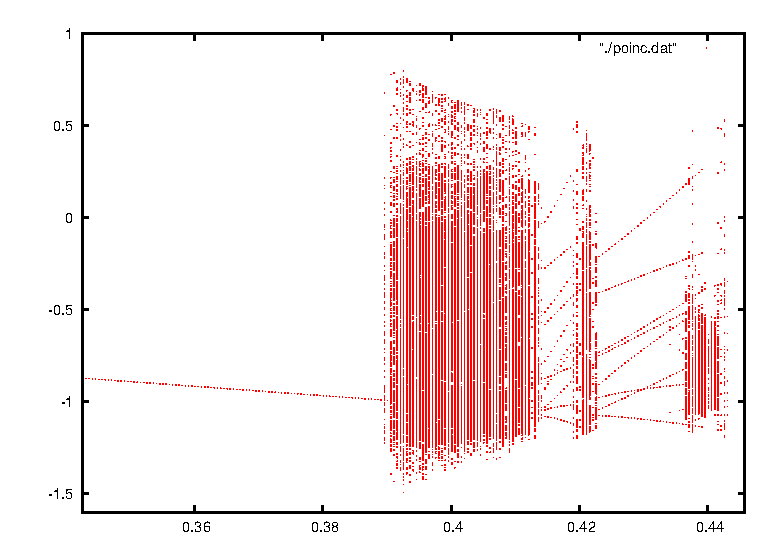
\includegraphics[width=0.9\columnwidth]{poinc-bf-f}
\end{center}
\end{figure}
\end{frame}

\begin{frame}[label=homogen-evol]
\begin{eqnarray}
M(t)=\frac{e^{-\gamma t/2}}{\omega_g}
\begin{pmatrix}
\omega_g\cos{\omega_g t}+\frac{\gamma}{2}\sin{\omega_g t} & \sin{\omega_g t}\\
-k\sin{\omega_g t} & \omega_g\cos{\omega_g t}-\frac{\gamma}{2}\sin{\omega_g t}
\end{pmatrix}
\end{eqnarray}

$(\omega_g=\frac{\sqrt{4k-\gamma^2}}{2})$
\hyperlink{BackFromM}{\beamergotobutton{Back}}
\end{frame}

\end{document}
